\documentclass[epsfig,10pt,fullpage]{article}

\newcommand{\LabNum}{8}
\newcommand{\CommonDocsPath}{../../../../common/docs}
\addtolength{\textwidth}{1.5in}
\addtolength{\oddsidemargin}{-0.75in}
\addtolength{\topmargin}{-0.75in}
\addtolength{\textheight}{1.5in}
\addtolength{\evensidemargin}{0.75in}
\setlength\parindent{0pt}
\raggedbottom

\usepackage{ae,aecompl}
\usepackage{epsfig,float,times}
\usepackage[hypcap]{caption}
\usepackage[pdftex, colorlinks]{hyperref}
\usepackage{graphicx}
\usepackage[usenames, dvipsnames]{color}
\usepackage{rotating}
\usepackage{tikz}
\usetikzlibrary{automata,positioning}
\usepackage{placeins}

\widowpenalty 10000
\clubpenalty 10000

\newcommand{\red}[1]{{\color{red}\sf{#1}}}
\newcommand{\green}[1]{{\color{green}\sf{#1}}}
\newcommand{\blue}[1]{{\color{blue}\sf{#1}}}
\definecolor{PineGreen}{rgb}{0.0, 0.47, 0.44}
\definecolor{ForestGreen}{rgb}{0.13, 0.55, 0.13}
\definecolor{Brown}{rgb}{0.59, 0.29, 0.0}

\newcommand{\UPDatePublished}{Oct 2021}
\newcommand{\versnum}{21.1} %version number quartus/AMP
\newcommand{\quartusname}{Quartus\textsuperscript{\textregistered} Prime}	
\newcommand{\UPTextBar}{For \quartusname{} \versnum{}}
\newcommand{\thisyear}{2021 } %for copyright
\newcommand{\company}{FPGAcademy.org}
\newcommand{\longteamname}{FPGAcademy.org}
\newcommand{\teamname}{FPGAcademy}
\newcommand{\website}{FPGAcademy.org}

\newcommand{\productAcronym}{AMP}
\newcommand{\productNameShort}{Monitor Program}

\newcommand{\productNameMedTM}{A Monitor Program}
\newcommand{\productNameMed}{A Monitor Program}

%\newcommand{\headerLogoFilePath}[1]{#1/FPGAcademy.png}

% listings is a package that supports encapsulating source code in LaTeX conveniently
\usepackage{listings}

\def\expandparam\lstinputlisting[#1]#2{\edef\tmp{\noexpand\lstinputlisting[#1]{#2}}\tmp}

%%%%%%%%%%%%%%%%%%%% Source Code Formatting %%%%%%%%%%%%%%%%%%%%
\definecolor{globalCommentColour}{rgb}{0.588,0.588,0.588}

%%%%%%%%%%%%%%%%%%%%%%%%%%%%%%%%%%%%%%%%%%%%%%%%%%%%
% Defining language style
% NiosII ASM
\lstdefinelanguage[NiosII]{Assembler} {
  morekeywords={add, addi, and, andhi, andi, beq, bge, bgeu, bgt, bgtu, ble,  bleu, blt, bltu, bne, br, break,
  bret, call, callr, cmpeq, cmpeqi, cmpge, cmpgei, cmpgeu, cmpgeui, cmpgt, cmpgti, cmpgtu, cmpgtui, cmple,
  cmplei, cmpleu, cmpleui, cmplt, cmplti, cmpltu, cmpltui, cmpne, cmpnei, custom, div, divu, eret, flushd,
  flushda, flushi, flushp, initd, initda, initi, jmp, jmpi, ldb, ldbio, ldbu, ldbuio, ldh, ldhio, ldhu, ldhuio,
  ldw, ldwio, mov, movhi, movi, movia, movui, mul, muli, mulxss, mulxsu, mulxuu, nextpc, nop, nor, or, orhi, ori,
  rdctl, rdprs, ret, rol, roli, ror, sll, slli, sra, srai, srl, srli, stb, stbio, sth, sthio, stw, stwio,
  sub, subi, sync, trap, wrctl, wrtcl, wrprs, xor, xori, xorhi, xori},
  morekeywords=[2]{.abort, .ABORT, .align, .app-file, .ascii, .asciz, .balign, .byte, .comm, .data, .def,
  .desc, .dim, .double, .eject, .else, .end, .endef, .endif, .equ, .equiv, .err, .extern, .file, .fill, .float,
  .global, .globl, .hword, .ident, .if, .include, .int, .irp, .irpc, .lcomm, .lflags, .line, .linkonce, .ln,
  .list, .long, .macro, .mri, .nolist, .octa, .org, .p2align, .psize, .quad, .rept, .sbttl, .scl, .section,
  .set, .short, .single, .size, .sleb128, .skip, .space, .stadb, .stabn, .stabs, .string, .symver, .tag,
  .text, .title, .type, .val, .uleb128, .word},
  morekeywords=[3]{et, bt, gp, sp, fp, ea, sstatus, ra, pc, status, estatus, bstatus, ienable, ipending, cpuid,
  exception, pteaddr, tlbacc, tlbmisc, eccinj, badaddr, config, mpubase, mpuacc},
  sensitive=t,
  alsoletter=.,
  morestring=[b]",
  morecomment=[s]{/*}{*/},
  morecomment=[l]\#,
}[keywords,comments,strings]
   
%% NOTE: morekeywords=[2] are GNU directives.
   
\definecolor{niosInstructionColour}{rgb}{0.000,0.608,0.000}
\definecolor{niosDirectiveColour}{rgb}{0.000,0.000,0.902}
\definecolor{niosSpecialRegColour}{rgb}{0.000,0.000,0.000}
\definecolor{niosStringColour}{rgb}{0.808,0.482,0.000}
   
%% NOTE: To make bold use: =\bfseries\color{<colour>}
\lstdefinestyle{defaultNiosStyle} {
  language=[NiosII]{Assembler},
  stringstyle=\color{niosStringColour},
  keywordstyle=\color{niosInstructionColour},
  keywordstyle=[2]\color{niosDirectiveColour},
  keywordstyle=[3]\itshape\color{niosSpecialRegColour}
}
%%%%%%%%%%%%%%%%%%%%%%%%%%%%%%%%%%%%%%%%%%%%%%%%%%%%

%%%%%%%%%%%%%%%%%%%%%%%%%%%%%%%%%%%%%%%%%%%%%%%%%%%%
% Defining language style
% ArmA9 ASM
\lstdefinelanguage[ArmA9]{Assembler} {
  morekeywords={ADC, ADD, ADDS, AND, ANDS, B, BAL, BEQ, BGE, BGT, BL, BLT, BIC, BKPT, BLX, BNE, BX, CDP, CLZ, CMN, CMP, EOR,
  EORS, LDC, LDM, LDR, LDRB, LDRBT, LDRH, LDRSB, LDRSH, LDRT, LSL, MCR, MLA, MOV, MOVW, MOVT, MRC, MRS, MSR, MUL, MVN, ORR, PLD,
  ROR, RSB, RSC, SBC, SMLAL, SMULL, STC, STM, STR, STRB, STRBT, STRH, STRT, SUB, SUBS, SWI, SWP, SWPB, TEQ, UMLAL,
  PUSH, POP, MOVS, RORS, LSR},
  morekeywords=[2]{.abort, .ABORT, .align, .app-file, .ascii, .asciz, .balign, .byte, .comm, .data, .def,
  .desc, .dim, .double, .eject, .else, .end, .endef, .endif, .equ, .equiv, .err, .extern, .file, .fill, .float,
  .global, .globl, .hword, .ident, .if, .include, .int, .irp, .irpc, .lcomm, .lflags, .line, .linkonce, .ln,
  .list, .long, .macro, .mri, .nolist, .octa, .org, .p2align, .psize, .quad, .rept, .sbttl, .scl, .section,
  .set, .short, .single, .size, .sleb128, .skip, .space, .stadb, .stabn, .stabs, .string, .symver, .tag,
  .text, .title, .type, .val, .vectors, .uleb128, .word},
  morekeywords=[3]{SP, PC, MIDR, CTR, TCMTR, TLBTR, MPIDR, ID_PFR0, ID_PFR1, ID_DFR0, ID_MMFR0, ID_MMFR1, ID_MMFR2,
  ID_MMFR3, ID_ISAR0, ID_ISAR1, ID_ISAR2, ID_ISAR3, ID_ISAR4, CCSIDR, CLIDR, AIDR, CSSELR, TTBR0, TTRB1, TTBR2, DACR,
  DFSR, IFSR, ADFSR, AIFSR, DFAAR, IFAR, ICIALLUIS, BPIALLIS, PAR, ICIALLU, ICIMVAU, BPIALL, DCIMVAC, DCISW, V2PCWPR,
  DCCVAC, DCCSW, DDIMVAC, DCISW, TLBALLIS, TLBIMVAIS, TLBIASIDIS, TLBIMVAAIS, TLBIALL, TLBIMVA, TLBIASID, TLBIMVAA,
  PMCR, PMCNTENSET, PMCNTENCLR, PMOVSR, PMSWINC, PMSELR, PMXEVTYPER, PMXEVCNTR, PMUSERENR, PMINTENSET, PMINTENCLR,
  PRRR, NRRR, PLEIDR, PLEASR, PLEFSR, PLEUAR, PLEPCR, VBAR, MVBAR, ISR, FCSEIDR, CONTEXTIDR, TPIDRURW, TPIDRURO, TPIDRPRW},
  sensitive=f,
  alsoletter=.,
  morestring=[b]",
  morecomment=[s]{/*}{*/},
  morecomment=[l]{//},
}[keywords,comments,strings]
   
%% NOTE: morekeywords=[2] are GNU directives.
   
\definecolor{armInstructionColour}{rgb}{0.000,0.608,0.000}
\definecolor{armDirectiveColour}{rgb}{0.000,0.000,0.902}
\definecolor{armSpecialRegColour}{rgb}{0.000,0.000,0.000}
\definecolor{armStringColour}{rgb}{0.808,0.482,0.000}
   
\lstdefinestyle{defaultArmStyle} {
  language=[ArmA9]{Assembler},
  stringstyle=\color{armStringColour},
  keywordstyle=\color{armInstructionColour},
  keywordstyle=[2]\color{armDirectiveColour},
  keywordstyle=[3]\itshape\color{armSpecialRegColour}
}
%%%%%%%%%%%%%%%%%%%%%%%%%%%%%%%%%%%%%%%%%%%%%%%%%%%%

%%%%%%%%%%%%%%%%%%%%%%%%%%%%%%%%%%%%%%%%%%%%%%%%%%%%
% Defining language style
% FPGAcademy ASM
\lstdefinelanguage{ASM}{
  morekeywords = [1]{mv, mvt, mvne, mvcc, add, sub, st, ld, and, b, bne, beq, bcc, bcs},
  morekeywords = [2]{word, define},
  keywordstyle = [1]\color{ForestGreen},
  keywordstyle = [2]\color{blue},
  sensitive = true,
  morecomment = [l]{//},
}

\lstset{
  language = ASM,
  basicstyle=\small\color{black}\ttfamily,
  commentstyle=\small\color{Brown}\itshape\ttfamily,
  showstringspaces=false,
  frame=none, %lines % boxed listings
  breaklines=true,
  breakatwhitespace=true,
  tabsize=3
}
%%%%%%%%%%%%%%%%%%%%%%%%%%%%%%%%%%%%%%%%%%%%%%%%%%%%

%%%%%%%%%%%%%%%%%%%%%%%%%%%%%%%%%%%%%%%%%%%%%%%%%%%%
% Defining language style
% Java
\definecolor{javaStringColour}{rgb}{0.808,0.482,0}
%%%%%%%%%%%%%%%%%%%%%%%%%%%%%%%%%%%%%%%%%%%%%%%%%%%%

%%%%%%%%%%%%%%%%%%%%%%%%%%%%%%%%%%%%%%%%%%%%%%%%%%%%
% Defining language style
% C
\definecolor{CStringColour}{rgb}{0.808,0.482,0}

\lstset{
  language = C,
  basicstyle=\small\color{black}\ttfamily, 
  commentstyle=\small\color{PineGreen}\itshape\ttfamily,
  keywordstyle=\small\color{blue}\bfseries\ttfamily,
  showstringspaces=false,
  frame=none, %lines % boxed listings
  breaklines=true,
  breakatwhitespace=true,
  tabsize=3
}
%%%%%%%%%%%%%%%%%%%%%%%%%%%%%%%%%%%%%%%%%%%%%%%%%%%%

%%%%%%%%%%%%%%%%%%%%%%%%%%%%%%%%%%%%%%%%%%%%%%%%%%%%
% Defining language style
% Verilog
\definecolor{verilogCommentColour}{rgb}{0.000,0.502,0.000}

\lstdefinestyle{defaultVerilogStyle} {
  language={Verilog},
  keywordstyle=\color{blue},
  commentstyle=\color{verilogCommentColour}
}
%%%%%%%%%%%%%%%%%%%%%%%%%%%%%%%%%%%%%%%%%%%%%%%%%%%%

%%%%%%%%%%%%%%%%%%%%%%%%%%%%%%%%%%%%%%%%%%%%%%%%%%%%
% Defining language style
% VHDL
\lstdefinestyle{defaultVHDLStyle} {
  language={VHDL},
  keywordstyle=\color{blue},
  commentstyle=\color{verilogCommentColour}
}
%%%%%%%%%%%%%%%%%%%%%%%%%%%%%%%%%%%%%%%%%%%%%%%%%%%%

%%%%%%%%%%%%%%%%%%%%%%%%%%%%%%%%%%%%%%%%%%%%%%%%%%%%
% Defining language style
% LaTeX
\lstdefinelanguage[LocalLaTeX]{TeX}[LaTeX]{TeX}{moretexcs={bf, it, sf, lstset},}

\lstdefinestyle{defaultLocalLatexStyle} {
  language=[LocalLatex]{TeX},
  keywordstyle=\color{blue}\bfseries,
  keywordstyle=[2]\color{blue},
  keywordstyle=[3]\color{blue}\bfseries
}
%%%%%%%%%%%%%%%%%%%%%%%%%%%%%%%%%%%%%%%%%%%%%%%%%%%%

%%%%%%%%%%%%%%%%%%%%%%%%%%%%%%%%%%%%%%%%%%%%%%%%%%%%
% Defining language style
% Default
\lstset{
  basicstyle=\small\color{black}\ttfamily,
  commentstyle=\small\color{globalCommentColour}\itshape\ttfamily,
  keywordstyle=\small\color{blue}\bfseries\ttfamily,
  showstringspaces=false,
  frame=none, %lines % boxed listings
  breaklines=true,
  breakatwhitespace=true,
  tabsize=3
}
%%%%%%%%%%%%%%%%%%%%%%%%%%%%%%%%%%%%%%%%%%%%%%%%%%%%


\hypersetup{
  pdftitle={Computer Organization Lab Exercise \LabNum},
  linkcolor=blue,
  hyperindex=true,
  pdfauthor={FPGAcademy.org},
  pdfkeywords={FPGAcademy.org, FPGAcademy, Lab, Exercise, Computer Organization},
  bookmarks,
  bookmarksopen=false,
  filecolor=blue,
  pdfstartview={FitH},
  urlcolor=blue,
  plainpages=false,
  pdfpagelabels=true,
  linkbordercolor={1 1 1} %no color for link border
}



\begin{document}

\centerline{\huge Computer Organization}
~\\
\centerline{\huge Laboratory Exercise \LabNum}
~\\
\centerline{\large Using Interrupts with Assembly Language and C code}
~\\

\noindent
The purpose of this exercise is to investigate the use of interrupts for the ARM* A9
processor, using both assembly language and C code. To do this exercise you need to be familiar 
with the exceptions processing mechanisms of the ARM processor, and with the operation of
the ARM Generic Interrupt Controller (GIC). These concepts are discussed in the tutorials 
{\it Introduction to the ARM Processor}, and {\it Using the ARM Generic Interrupt
Controller}. We assume that you are using either the DE1-SoC or DE10-Standard Computer to 
implement the solutions to this exercise. It may be useful to read the documentation for
these computer systems that pertains to the use of exceptions and interrupts.

~\\
\noindent
{\bf Part I}
~\\
~\\
\noindent
Consider the main program shown in Figure~\ref{fig:code}. The code first specifies the
exceptions vector table for the ARM processor using a code section called .{\it vectors}.
Only the IRQ vector is set up for this program. The .{\bf word} Assembler directive is used to 
create placeholders (0's) for all of the vectors except IRQ, which is 
set to branch to an interrupt service routine called SERVICE\_IRQ.  
In the .{\it text} section of the main program the stack pointers, for both 
interrupt mode and supervisor mode, are initialized, the generic interrupt controller
(GIC) is configured, and the pushbutton KEYs port is set up to generate interrupts.
Finally, the main program enables interrupts in the processor.  You are to fill in the code that 
is not shown in the figure.  

~\\
\noindent
The main program in Figure~\ref{fig:code} consists of an endless loop that comprises 
a few logical instructions. The code in this loop does not serve any useful purpose other 
than to provide a specific set of instructions that are being executed repeatedly: logical
AND, Exclusive-OR, logical OR, and branch. When a pushbutton KEY is pressed to cause an 
interrupt, the main program may be executing any of the instructions in the loop. After 
this instruction is completed, the processor will branch to the interrupt handler. 
Figure~\ref{fig:handler} shows most of the code for the interrupt handler. It passes to 
the KEYs interrupt service routine, as a parameter in register R0, the machine code 
of the next instruction to be executed in the main program. You have to write the KEYs interrupt 
service routine. It should display on the Terminal window of the Monitor Program which 
instruction will be executed when the processor returns to the main program. 
An example of output on the Terminal window after several KEY presses might be:

~\\
\begin{minipage}[t]{12.5 cm}
\begin{lstlisting}
AND
ORR
B
EOR
EOR
AND
...
\end{lstlisting}
\end{minipage}

\begin{figure}[H]
\begin{center}
\lstinputlisting[style=defaultArmStyle]{../design_files/part1.s}
\end{center}
\caption{Main program and interrupt service routine.}
\label{fig:code}
\end{figure}

\noindent
Perform the following:

\begin{enumerate}
\item Create a new folder to hold your solution for this part. Create a
file, such as {\it part1.s}, and type the assembly language code for the main program 
into this file. 

\item Create any other source code files you may want, and write the code for the
{\it CONFIG\_GIC} subroutine that initializes the GIC. Set up the GIC to send interrupts
to the ARM processor from the pushbutton KEYs port. 

\begin{figure}[t]
\begin{center}
\lstinputlisting[style=defaultArmStyle]{../design_files/exception_handler.s}
\end{center}
\caption{The IRQ Exception handler.}
\label{fig:handler}
\end{figure}

\item 
To implement the KEYs interrupt service routine, you need to know the ARM
instruction-encodings that are shown in Figure~\ref{fig:encoding}.  Part $a$ of the figure 
gives the encoding of data processing instructions, which include AND, EOR, and 
ORR, and Figure~\ref{fig:encoding}$b$ displays the encoding of branch instructions. 
For all of the relevant instructions used here the {\sf Cond} 
field will have the value {\sf 1110}, which 
represents the condition {\it always}.  In part $a$ of Figure~\ref{fig:encoding}
the {\sf I} field indicates an {\it immediate} operand. This field is~1 if {\it Operand2}
is an immediate constant, otherwise 0. The {\sf OpCode} field specifies the type of data
processing instruction: it has the values {\sf 0000} for AND, {\sf 0001} for EOR and 
{\sf 1100} for ORR. The {\sf S} bit is 1 if the instruction modifies the condition codes, 
otherwise 0. Fields {\sf Rn} and {\sf Rd} specify the first operation register and destination 
register, respectively.  Field {\sf Operand2} specifies the {\it flexible} second operand. When 
a register is used for this operand, it is identified in bits $3-0$. In 
Figure~\ref{fig:encoding}$b$ the {\sf L} bit is 0 for a Branch instruction and 1 for 
Branch-with-link.  The {\sf offset} field is a 24-bit signed number in 2's complement format.

~\\
\begin{figure}[htb]
	\begin{center}
	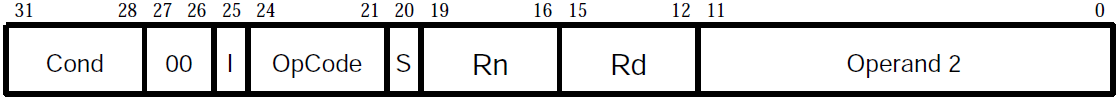
\includegraphics[width=5in]{figures/encodingDataProcess.png}

	~\\
	{\sf (a) Data processing instructions}

	~\\
	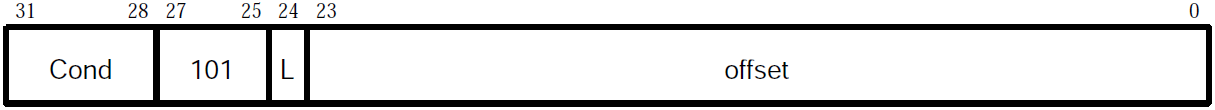
\includegraphics[width=5in]{figures/encodingB.png}

	~\\
	{\sf (b) Branch instructions}
	\end{center}
	\vspace{-0.25cm}\caption{The machine code format.}
\label{fig:encoding}
\end{figure}

\newpage
To display the name of an instruction mnemonic on the Terminal window you may wish to 
declare some strings of data as indicated below, and write the characters in these strings to the 
JTAG* UART that is connected to the Terminal window:

\begin{minipage}[t]{12.5 cm}
\begin{lstlisting}[style=defaultArmStyle]
AND: 		.asciz 	"AND\n"
ORR: 		.asciz 	"ORR\n"
EOR: 		.asciz 	"EOR\n"
BAL: 		.asciz 	"B\n"
\end{lstlisting}
\end{minipage}

\item
Make a new Monitor Program project in the folder where you stored your source-code files.
In the Monitor Program screen illustrated in Figure~\ref{fig:exceptions}, 
choose {\sf Exceptions} in the {\it Linker Section Presets} drop-down menu.
In the screen of Figure~\ref{fig:terminal}, select {\sf JTAG\_UART\_for\_ARM\_0} as 
the {\it Terminal device}.  Refer to Exercise 2, Part IV, for information on using 
the JTAG UART to communicate with the Monitor Program's Terminal window.  

\item
Compile, download, and test your program.
\end{enumerate}

~\\
\begin{figure}[H]
	\begin{center}
	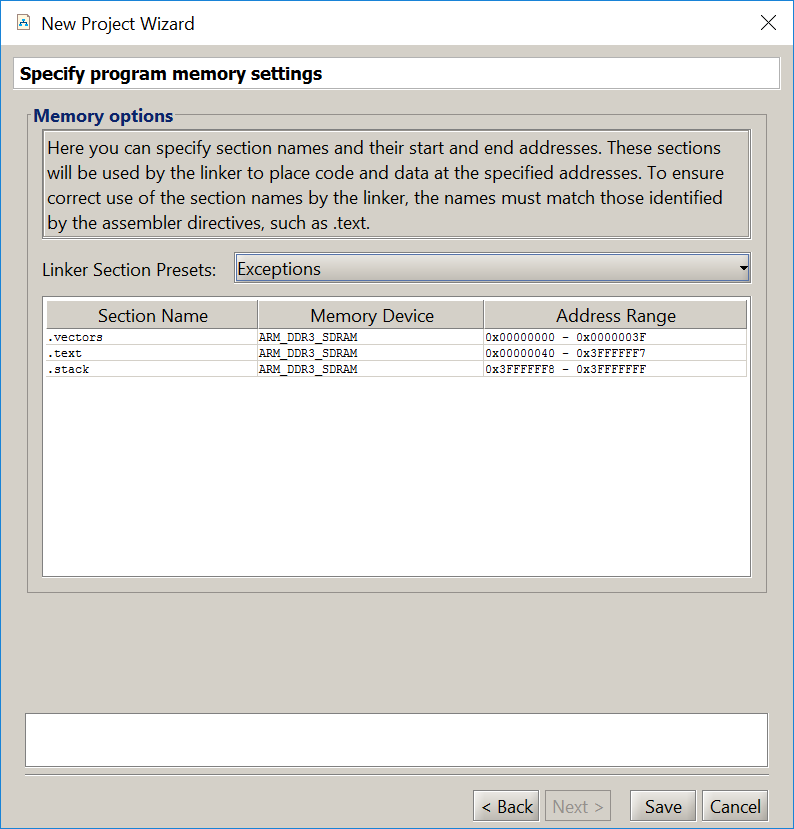
\includegraphics[scale=0.8]{figures/exceptions_s.png}
	\end{center}
	\vspace{-0.25cm}\caption{Selecting the {\sf Exceptions} linker section.}
\label{fig:exceptions}
\end{figure}
\newpage

\begin{figure}[htb]
	\begin{center}
	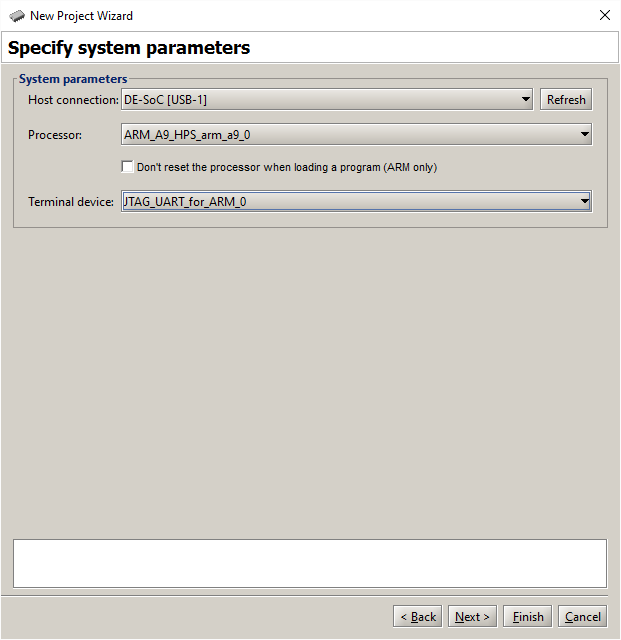
\includegraphics[scale=0.58]{figures/terminal.png}
	\end{center}
	\vspace{-0.25cm}\caption{Specifying the {\it Terminal device}.}
\label{fig:terminal}
\end{figure}

\noindent
{\bf Part II}
~\\
~\\
For this part you are to modify your code from Part I so that additional information is
displayed on the Terminal window when a pushbutton KEY is pressed. All of your changes for
this part should be done in the interrupt service routine for the pushbutton KEYs. You
should not have to change any other files. For Part I you were required to display only 
the mnemonic of the next instruction, such as AND or EOR, that is to be executed in the
main program on return from an interrupt. For this part you are to extend your solution
so that it also displays the names of the register arguments of each instruction. Use the
machine encodings shown in Figure~\ref{fig:encoding} to find the required information. An 
example of output produced on the Terminal window after several KEYs have been pressed
might be:

~\\
\begin{minipage}[t]{12.5 cm}
\begin{lstlisting}
ORR 	R2, R1, R0
EOR 	R3, R4, R5
AND 	R0, R1, R2
B 		0xFFFFF8
ORR 	R6, R7, R8
AND 	R8, R7, R6
...
\end{lstlisting}
\end{minipage}

~\\
~\\
For logical instructions you can assume that only the register numbers used 
in the main program from Figure~\ref{fig:code} have to be supported. Thus, your code only has to 
be able to display register indices which are single-digit numbers from 0 to 9. For a
branch instruction you are to show the 24-bit branch offset as a 2's-complement number, as
indicated in the example output that is provided above.

\noindent
{\bf Part III}
~\\
~\\
\noindent
Consider the C code shown in Figure~\ref{fig:C_code1}. It contains an endless loop that
repeatedly calls a function named {\it KEY\_pressed}, not shown in the figure, which 
checks to see if a KEY is
currently being pressed. If so, it waits for the KEY to be released and then returns 1. 
Otherwise, if no KEY was pressed, 0 is returned. When {\it KEY\_pressed} returns 1, the main
program calls a function named {\it doit}. This function is supposed to print, on the Terminal 
window, the mnemonic of the instruction that will be executed on return from the {\it doit}
function. In the main program {\it inline assembly} commands are used to insert specific
instructions following each call to {\it doit}. For example, the first call to {\it doit}
is followed by the instruction {\sf AND R0, R1, R2}, the second call to {\it doit} is
followed by the instruction {\sf EOR R3, R4, R5}, and so on.

~\\
\noindent
Part of the code for the {\it doit} function is given in Figure \ref{fig:C_code1}. It uses two
inline assembly commands. The command


\begin{center}
\begin{tabular}{c}
\begin{lstlisting}[language=C]
asm("LDR R0, [LR]" : : : "r0")
\end{lstlisting}
\end{tabular}
\end{center}

\noindent
loads the machine code of the instruction pointed to by the link register into register R0. The 
argument "r0" in this command informs the C compiler that the contents of register R0 will be 
changed as a result of executing the instruction. The command

\begin{center}
\begin{tabular}{c}
\begin{lstlisting}[language=C]
asm("MOV \%0, R0" : "=r" (machine_code) : : )
\end{lstlisting}
\end{tabular}
\end{center}

\noindent
copies the contents of register R0 into the variable {\it machine\_code}. The argument {\sf \%0}
in this command is set to whichever register, for example register R1, is chosen by the C
compiler to hold the value of the variable {\it machine\_code}.  

~\\
\noindent
Make sure that you understand how the inline assembly commands work. Documentation on
these commands can be found by searching on the web for {\it gnu inline assembly ARM}, or
something similar.

~\\
\noindent
Perform the following:

\begin{enumerate}
\item
Create a new folder to hold your solution to this part. 
Type the C code for the main program into a file, for example {\it part3.c}. Also, add
your own code for the {\it KEY\_pressed} function.

\item 
Complete the C code for the {\it doit} function. You should display on the Terminal window
the mnemonic of the instruction corresponding to the {\it machine\_code} variable.
Refer to Figure~\ref{fig:encoding} for the machine code formats.
You should use the {\it printf} library function to display the result produced by the program. 
To use the {\it printf} function include the {\it stdio.h} library as shown in
Figure~\ref{fig:C_code1}.

\item
Make a new Monitor Program project for this part of the exercise. In the Monitor Program screen 
shown in Figure~\ref{fig:MPterminal} set the {\it Terminal device} to {\sf Semihosting}.
This setting causes the output of library functions like {\it printf} to appear 
in the {\it Terminal} window of the Monitor Program graphical user interface.

\item
Compile, download, and test your program. 
\end{enumerate}

\begin{figure}[H]
\begin{center}
\lstinputlisting[language=C]{../design_files/part3.c}
\end{center}
\caption{Main program for Part III.}
\label{fig:C_code1}
\end{figure}

\newpage
\begin{figure}[htb]
	\begin{center}
	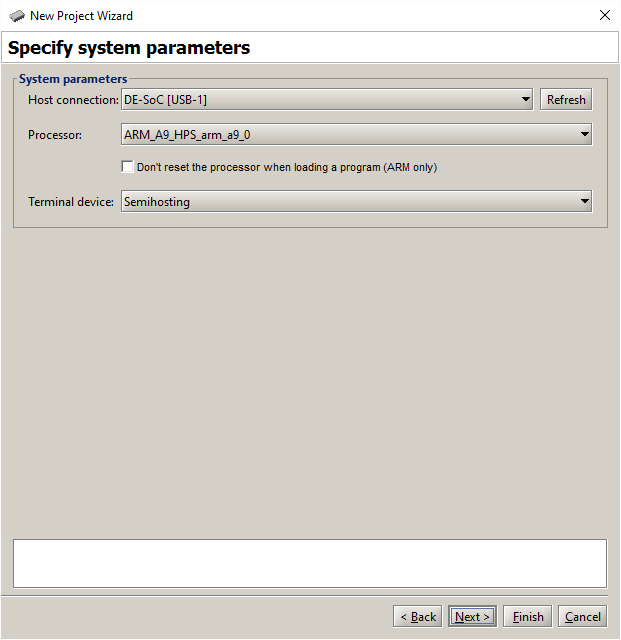
\includegraphics[scale=0.58]{figures/figureMP_terminal.png}
	\end{center}
	\vspace{-0.25cm}\caption{Specifying the {\it Terminal device}.}
\label{fig:MPterminal}
\end{figure}

~\\
~\\
\noindent
{\bf Part IV}
~\\
~\\
\noindent
In this part you are to repeat the tasks given in Parts I and II, but using C code rather
than assembly-language code.

~\\
\noindent
Consider the main program shown in Figure~\ref{fig:C_code2}. The program first initializes the
ARM A9 stack pointer for IRQ (interrupt) mode by calling a subroutine named
{\it set\_A9\_IRQ\_stack()}. This step is necessary because, although
the C compiler automatically generates code that initializes the SVC-mode (supervisor mode)
stack pointer, the C compiler does not generate code to initialize the IRQ-mode stack pointer.
The main program then calls subroutines {\it config\_GIC()} to initialize the generic 
interrupt controller (GIC), and {\it config\_KEYs()} to initialize the pushbutton KEYs 
port so that it will generate interrupts. 
Finally, a subroutine {\it enable\_A9\_interrupts()} is called to unmask
IRQ interrupts in the ARM processor.

~\\
\noindent
After completing the initialization steps
described above, the main program executes an endless loop that consists of several
logical instructions. Inline assembly commands, described in Part III, are used to specify 
the logic instructions.

\clearpage
\begin{figure}[H]
\begin{center}
\lstinputlisting[language=C]{../design_files/part4.c}
\end{center}
\caption{Main program for Part IV.}
\label{fig:C_code2}
\end{figure}

~\\
\noindent
Perform the following:

\begin{enumerate}
\item Create a new folder to hold your solution for this part. Create a
file, such as {\it part1.c}, for your main program, and create any other source-code files 
that you may wish to use.  Write the code for the subroutines that are called by the 
main program. For the {\it config\_GIC()} subroutine set up the
GIC to send interrupts to the ARM processor from the pushbutton KEYs port. 

\item 
Figure~\ref{fig:irq_code} gives part of the C code required for the interrupt handler. 
It is declared with the {\bf \_$\,$\_attribute\_$\,$\_} specification {\it interrupt}, 
and has the special name 
{\it \_$\,$\_cs3\_isr\_irq}.  Using this declaration allows the C compiler to recognize the 
code as being the IRQ interrupt handler. The compiler generates an entry that branches to
this code in the ARM exception-vector table. Complete the missing part of this code. You
have to obtain the machine code of the next instruction to be executed on return from the 
interrupt, and pass this machine code to the interrupt service routine for the
pushbutton KEYs.
  
You have to write the code for the {\it pushbutton\_isr()} interrupt service routine.
Your code should perform the same task as in Part II of this exercise. That is, you are to
print on the Terminal window the mnemonic, and register indices, of the instruction that 
will be executed on return from the interrupt. You can make the same assumptions as in
Parts I and II, namely that only the logical instructions, plus the branch instruction,
have to be handled by your code. For the branch instruction display the 24-bit branch
offset as its argument.

\item
Make a new Monitor Program project in the folder where you stored your source-code files.
As discussed for Part III, in the Monitor Program screen shown in 
Figure~\ref{fig:MPterminal} set the {\it Terminal device} to {\sf Semihosting}.
Also, in the Monitor Program screen illustrated in Figure~\ref{fig:exceptions}, make sure 
to choose {\sf Exceptions} in the {\it Linker Section Presets} drop-down menu.

\item
Compile, download, and test your program. 
\end{enumerate}

\begin{figure}[H]
\begin{center}
\lstinputlisting[language=C]{../design_files/exception_handler.c}
\end{center}
\caption{IRQ Exception handler.}
\label{fig:irq_code}
\end{figure}

~\\
\begin{figure}[htb]
	\begin{center}
	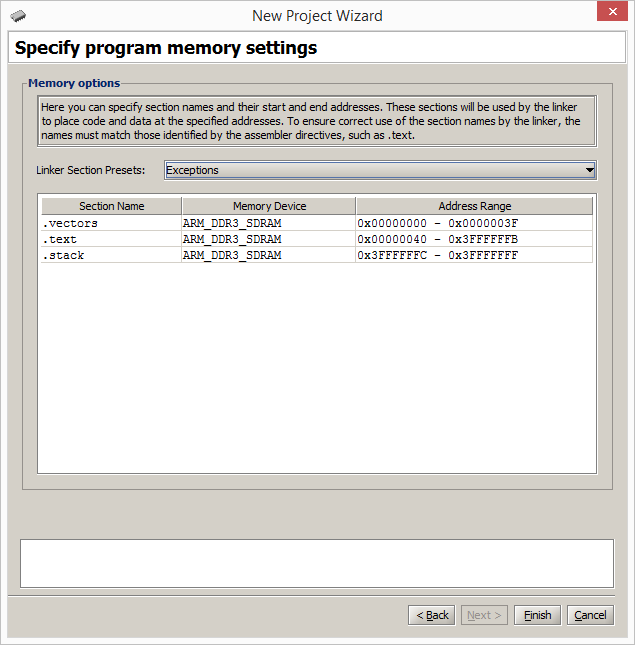
\includegraphics[scale=0.58]{figures/exceptions_C.png}
	\end{center}
	\vspace{-0.25cm}\caption{Selecting the {\sf Exceptions} linker section.}
\label{fig:exceptions}
\end{figure}


%%%%%%%%%%%%%%%%%%%%%%%%%%%%%%%%%%%%%%%%
%%% FPGAcademy Copyright Information %%%
%%%%%%%%%%%%%%%%%%%%%%%%%%%%%%%%%%%%%%%%

%Always put the copyright on a new page (clear page), with some vertical space from top
\clearpage
\vspace{1in}

\noindent

Copyright {\copyright} FPGAcademy.org. All rights reserved. FPGAcademy and the 
FPGAcademy logo are trademarks of FPGAcademy.org.  This document is provided 
"as is", without warranty of any kind, express or implied, including but not 
limited to the warranties of merchantability, fitness for a particular purpose 
and noninfringement. In no event shall the authors or copyright holders be 
liable for any claim, damages or other liability, whether in an action of 
contract, tort or otherwise, arising from, out of or in connection with the 
document or the use or other dealings in the document.
~\\
~\\
**Other names and brands may be claimed as the property of others.


\end{document}
